% Chapter 3

\chapter{The Quran Phonetic Script} % Main chapter title

\label{Chapter3} % For referencing the chapter elsewhere, use \ref{Chapter3} 

\lhead{Chapter 3. \emph{The Quran Phonetic Script}} % This is for the header on each page - perhaps a shortened title

%--------------------------------------------------------------

\section{Introudction}



We consider the Quran Phonetic Script to be the most valuable and important contribution of our work. By formalizing the assessment of Holy Quran pronunciation as an ASR problem represented through this script, we provide a comprehensive solution to the task.

\subsection{Motivation for Developing Quran Phonetic Script}

Modern Standard Arabic (MSA) orthography cannot adequately represent Tajweed rules for error detection. For example, MSA cannot measure the precise length of Madd rules. Previous research (e.g., \cite{omran2023automatic}) focused on single rules like Qalqalah. Our phonetic script addresses this limitation by capturing all Tajweed pronunciation errors except Ishmam (\arb{إشمام}), which involves a visual mouth movement without audible output.

\subsection{Background}

We based our script on classical Muslim scholarship rather than the International Phonetic Alphabet (IPA) for these reasons:

\begin{enumerate}
    \item \textbf{Historical Precedence}: Muslim scholars from the 6th to 14th centuries rigorously defined Quranic errors centuries before modern phonetics emerged in the West.
    \item \textbf{Scientific Foundation}: Scholars like Al-Khalil ibn Ahmad (6th century AH) systematically described articulations and attributes with remarkable accuracy comparable to modern phonetics \cite{article-khalil}.
    \item \textbf{Pedagogical Relevance}: Learners' errors align with classical definitions according to expert Quran teachers.
\end{enumerate}

\subsection{Defining Mistakes in Quran Recitation}

Following \cite{sweed2021}, Quran recitation errors fall into three categories:
\begin{enumerate}
    \item \textbf{Articulation Errors}: Incorrect pronunciation of phonemes
    \item \textbf{Attribute Errors}: Mistakes in letter characteristics (Sifat al-Huruf)
    \item \textbf{Tajweed Rule Errors}: Incorrect application of rules like Ghunnah, Madd, etc.
\end{enumerate}

Our script comprehensively addresses all three aspects through two output levels:
\begin{itemize}
    \item \textbf{Phonemes Level}: Represents letters, vowels, and Tajweed rules
    \item \textbf{Sifat Level}: Represents articulation attributes for each phoneme
\end{itemize}

\subsection{Phoneme Set (43 Symbols)}

\begin{longtable}{|l|l|l|}
\caption{The table shows our defening for the phonemes level for the Quran Phonetic Script by (43) phonemes.}
\label{table:table_phonemes_level_def}
\hline
\textbf{Phoneme Name} & \textbf{Symbol} & \textbf{\arb{الحرف  بالعربية}} \\ \hline
\hline
\endfirsthead
\multicolumn{3}{c}%
{{\bfseries \tablename\ \thetable{} -- continued from previous page}} \\ \hline
\textbf{Phoneme Name} & \textbf{Symbol} & \textbf{\arb{الحرف  بالعربية}} \\ \hline
\endhead
hamza & \arb{ء} & \arb{همزة} \\ \hline
baa & \arb{ب} & \arb{باء} \\ \hline
taa & \arb{ت} & \arb{تاء} \\ \hline
thaa & \arb{ث} & \arb{ثاء} \\ \hline
jeem & \arb{ج} & \arb{جيم} \\ \hline
haa\_mohmala & \arb{ح} & \arb{حاء} \\ \hline
khaa & \arb{خ} & \arb{خاء} \\ \hline
daal & \arb{د} & \arb{دال} \\ \hline
thaal & \arb{ذ} & \arb{ذال} \\ \hline
raa & \arb{ر} & \arb{راء} \\ \hline
zay & \arb{ز} & \arb{زاي} \\ \hline
seen & \arb{س} & \arb{سين} \\ \hline
sheen & \arb{ش} & \arb{شين} \\ \hline
saad & \arb{ص} & \arb{صاد} \\ \hline
daad & \arb{ض} & \arb{ضاد} \\ \hline
taa\_mofakhama & \arb{ط} & \arb{طاء} \\ \hline
zaa\_mofakhama & \arb{ظ} & \arb{ظاء} \\ \hline
ayn & \arb{ع} & \arb{عين} \\ \hline
ghyn & \arb{غ} & \arb{غين} \\ \hline
faa & \arb{ف} & \arb{فاء} \\ \hline
qaf & \arb{ق} & \arb{قاف} \\ \hline
kaf & \arb{ك} & \arb{كاف} \\ \hline
lam & \arb{ل} & \arb{لام} \\ \hline
meem & \arb{م} & \arb{ميم} \\ \hline
noon & \arb{ن} & \arb{نون} \\ \hline
haa & \arb{ه} & \arb{هاء} \\ \hline
waw & \arb{و} & \arb{واو} \\ \hline
yaa & \arb{ي} & \arb{ياء} \\ \hline
alif & \arb{ا} & \arb{نصف مد ألف} \\ \hline
yaa\_madd & \arb{ۦ} & \arb{نصف مد ياء} \\ \hline
waw\_madd & \arb{ۥ} & \arb{نصف مد واو} \\ \hline
fatha & \arb{َ} & \arb{فتحة} \\ \hline
dama & \arb{ُ} & \arb{ضمة} \\ \hline
kasra & \arb{ِ} & \arb{كسرة} \\ \hline
fatha\_momala & \arb{۪} & \arb{فتحة ممالة} \\ \hline
alif\_momala & \arb{ـ} & \arb{ألف ممالة} \\ \hline
hamza\_mosahala & \arb{ٲ} & \arb{همزة مسهلة} \\ \hline
qlqla & \arb{ڇ} & \arb{قلقة} \\ \hline
noon\_mokhfah & \arb{ں} & \arb{نون مخفاة} \\ \hline
meem\_mokhfah & \arb{۾} & \arb{ميم مخفاة} \\ \hline
sakt & \arb{ۜ} & \arb{سكت} \\ \hline
dama\_mokhtalasa & \arb{ؙ} & \arb{ضمة مختلسة (عند الروم في تأمنا)} \\ \hline
\end{longtable}

\subsection{Sifat (Attributes) (10)}

\begin{longtable}{|l|l|l|l|}
\caption{The table showes sefining 14 sifa (\arb{صفة}) as 10 levels.}
\label{table:table_sifa_level_def}
\hline
\textbf{Sifat (English)} & \textbf{Sifat (Arabic)} & \textbf{Values (English)} & \textbf{Values (Arabic)} \\ \hline
\endfirsthead
\multicolumn{4}{c}%
{{\bfseries \tablename\ \thetable{} -- continued from previous page}} \\ \hline
\textbf{Sifat (English)} & \textbf{Sifat (Arabic)} & \textbf{Values (English)} & \textbf{Values (Arabic)} \\ \hline
\endhead
hams\_or\_jahr & \arb{الهمس أو الجهر} & hams, jahr & \arb{همس, جهر} \\ \hline
shidda\_or\_rakhawa & \arb{الشدة أو الرخاوة} & shadeed, between, rikhw & \arb{شديد, بين بين, رخو} \\ \hline
tafkheem\_or\_taqeeq & \arb{التفخيم أو الترقيق} & mofakham, moraqaq, low\_mofakham & \arb{مفخم, مرقق, أدنى المفخم} \\ \hline
itbaq & \arb{الإطباق} & monfateh, motbaq & \arb{منفتح, مطبق} \\ \hline
safeer & \arb{الصفير} & safeer, no\_safeer & \arb{صفير, لا صفير} \\ \hline
qalqla & \arb{القلقلة} & moqalqal, not\_moqalqal & \arb{مقلقل, غير مقلقل} \\ \hline
tikraar & \arb{التكرار} & mokarar, not\_mokarar & \arb{مكرر, غير مكرر} \\ \hline
tafashie & \arb{التفشي} & motafashie, not\_motafashie & \arb{متفشي, غير متفشي} \\ \hline
istitala & \arb{الاستطالة} & mostateel, not\_mostateel & \arb{مستطيل, غير مستطيل} \\ \hline
ghonna & \arb{الغنة} & maghnoon, not\_maghnoon & \arb{مغنون, غير مغنون} \\ \hline
\end{longtable}

\subsection{Development Methodology}

\begin{enumerate}
    \item \textbf{Imlaey to Uthmani Conversion}: where convert Imlaey Script to Uthmani Script as we rely on Uthmani script to construct Quran Phoneme Script.
    \item \textbf{Uthmani to Phonetic Script Conversion}: where we convert Uthmani Script to Quran Phonetic Script.
\end{enumerate}





% --------------------------------------------------------------------------------------------------------------



\section{Converting Imlaey Script to Uthmani Script}

As mentioned, we selected the Uthmani script as our foundation because:
\begin{itemize}
\item It contains specialized Tajweed diacritics (Madd, Tasheel, etc.).
\item It preserves pause rules critical for recitation (e.g., stopping on \arb{رحمت}).
\end{itemize}

To facilitate this conversion, we created an annotation UI to manually annotate misaligned words between the two scripts. For example:

\begin{table}[H]
\centering
\begin{tabular}{|l|l|}
\hline
\textbf{Imlaey Script} & \textbf{Uthmani Script} \\
\hline
\arb{يَا ابْنَ أُمَّ} & \arb{يَبْنَؤُمَّ} \\
\hline
\end{tabular}
\caption{Example of script alignment}
\label{tab:example1}
\end{table}

Subsequently, we developed an algorithm that relies on these annotations to convert Imlaey to Uthmani.

\subsection{Annotation Platform}

We developed an annotation application to map misaligned words between the Uthmani and Imlaey scripts. The platform consists of two components: a frontend using Streamlit\footnote{\url{https://streamlit.io/}} and a backend using FastAPI\footnote{\url{https://fastapi.tiangolo.com/}}. The core idea is to align words between the Imlaey and Uthmani scripts. We first loop over every ayah in both scripts; if we find a misalignment (where the number of Imlaey words is not equal to the number of Uthmani words), we prompt the user to align the words, as shown in the figure below.

\begin{figure}[H]
\centering
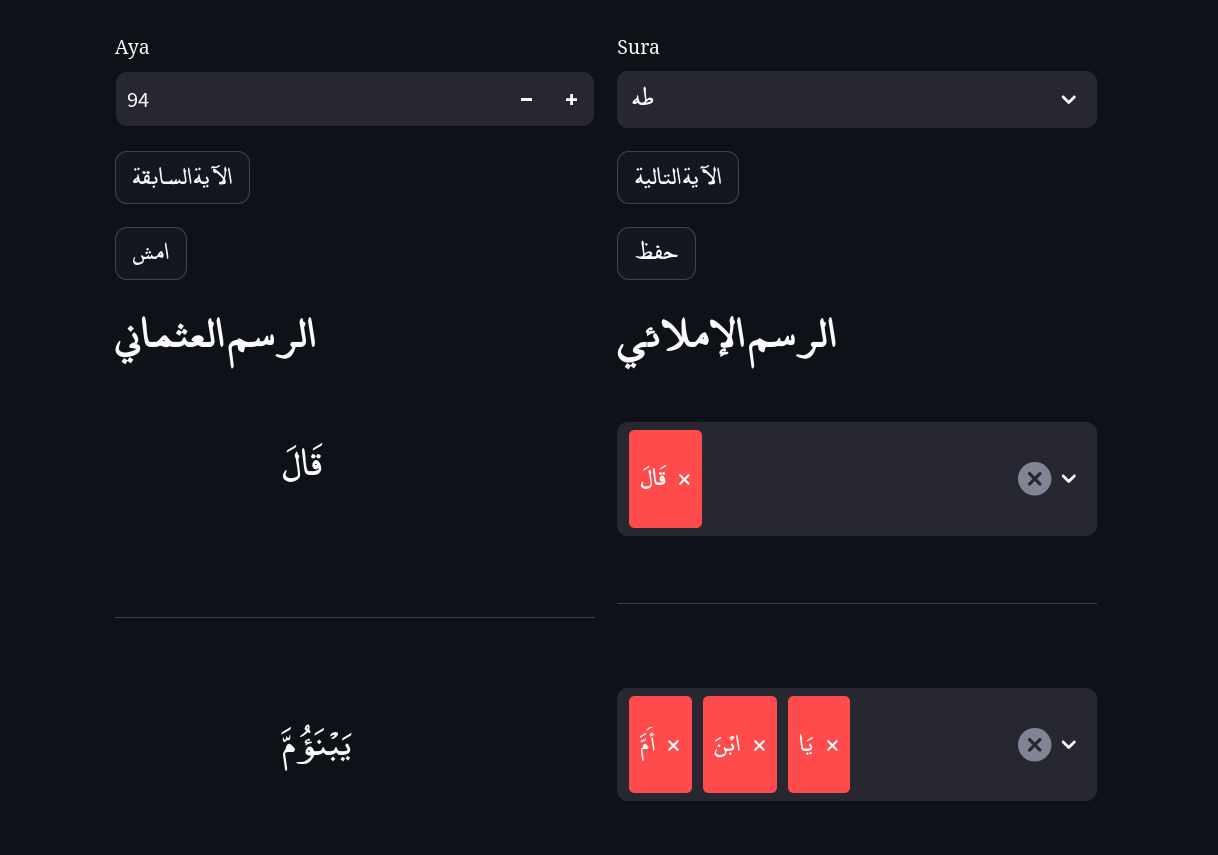
\includegraphics[width=0.8\textwidth]{../figures/imlaey-to-uthmani.png}
\caption{A screenshot of the UI where the user aligns words for both scripts.}
\label{fig:alignment-ui}
\end{figure}

\subsection{Observations}

After completing the annotation, we attempted to identify patterns of mismatches between the Imlaey and Uthmani scripts. We found the following patterns, as shown below:

\begin{table}[H]
\centering
\begin{tabular}{|l|l|l|}
\hline
\textbf{Imlaey Script} & \textbf{Uthmani Script} & \textbf{(Surah, Ayah)} \\
\hline
\arb{يَا ابْنَ أُمَّ} & \arb{يَبْنَؤُمَّ} & (20, 94) \\
\hline
\arb{وَأَن لَّوِ} & \arb{وَأَلَّوِ} & (72, 16) \\
\hline
\end{tabular}
\caption{Examples of script mismatches}
\label{tab:mismatches}
\end{table}

Specifically, we found that Imlaey words starting with certain patterns, along with the following word, map to a single Uthmani word.

\begin{table}[H]
\centering
\begin{tabular}{|l|l|}
\hline
\textbf{Imlaey Word Start} & \textbf{Count in the Holy Quran} \\
\hline
\arb{يَا} & 350 \\
\hline
\arb{وَيَا} & 11 \\
\hline
\arb{هَا} & 4 \\
\hline
\end{tabular}
\caption{Common Imlaey word patterns}
\label{tab:patterns}
\end{table}

\subsection{Imlaey to Uthmani Algorithm}

Based on these observations, we created an algorithm that performs a lookup for these patterns to align both scripts. This resulted in the \texttt{quran-transcript}\footnote{\url{https://github.com/obadx/quran-transcript}} Python package. With a simple \texttt{pip} installation command, the conversion is functional:


\begin{listing}[H]
\begin{minted}[escapeinside=``]{python}
from quran_transcript import search, Aya

imlaey_text = `\pythonarb{فأخرج به من الثمرات رزقا لكم}`
results = search(
    imlaey_text,
    start_aya=Aya(2, 13),
    window=20,
    remove_tashkeel=True
)

uthmani_script = results[0].uthmani_script
print(uthmani_script)
# Output: `\pythonarb{فَأَخْرَجَ بِهِۦ مِنَ ٱلثَّمَرَٰتِ رِزْقًۭا لَّكُمْ}`
\end{minted}
\caption{Usage example with escaped Arabic}
\label{code:example-escaped}
\end{listing}




% ------------------------------------------------------------------------------------------------------------


\section{Quran Phonetic Script Construction}

The Quran Phonetic Script is a set of letters and attributes (\arb{صفات}) that describes what the Holy Quran's reciters \textbf{actually} said. It was designed to capture all recitation rules, including all Tajweed rules (except Ishmam \arb{إشمام} and pausing with rawm \arb{روم} or \arb{إشمام}) and Sifat. This script is composed of 11 levels:

\begin{itemize}
\item \texttt{phonemes} level: Designed to capture pronunciation of letters like baa (\arb{ب}) and diaractization like (fatha, damma and kasra).
\item \texttt{sifat} level: Consisting of 10 levels to capture the attribute of articulation (\arb{صفة}) for every phoneme group.
\end{itemize}

We built this script based on \texttt{Hafs} (\arb{رواية حفص}) and incorporated all the different ways of reciting for \texttt{Hafs}. For example, the length of Madd Almunfasil can be (2, 3, 4, or 5 beats). Other variations can be found here \ref{sec:hafs_ways}.

\subsection{Phonemes Level}

The phoneme level has specific features, which are summarized as:

\begin{enumerate}
\item \textbf{Madd Representation}:
\begin{itemize}
\item Normal Madd appears as consecutive madd symbols (e.g., 4-beat Madd: \arb{اااا}).
\item Madd al-Leen is represented with multiple waw/yaa symbols.
\end{itemize}

\item \textbf{Ghunnah}:
\begin{itemize}
\item Stressed Ghunnah for noon (e.g., \arb{النون المشددة}) is represented as three consecutive noon symbols (\arb{ننن}).
\item Ikhfa is represented as three consecutive noon\_mokhfah (\arb{ںںں}) or meem\_mokhfah (\arb{۾۾۾}).
\end{itemize}

\item \textbf{Idgham Handling}:
\begin{itemize}
\item Idgham for sakin noon with yaa is represented by consonant doubling (e.g., \arb{مَن يَعْمَلْ} → \arb{مَنيييَعمَل}).
\end{itemize}

\item \textbf{Special Cases}:
\begin{itemize}
\item Sakin: No following vowel symbol.
\item Imala: Represented by fatha\_momala and alif\_momala.
\item Rawm: Represented by the dama\_mokhtalasa marker.
\end{itemize}
\end{enumerate}


\begin{table*}[h]
\centering
\caption{Examples of Uthmani to Phonetic Script Conversion with Sifat Attributes}
\label{tab:examples_with_sifat}
\scriptsize
\setlength{\tabcolsep}{3pt}
\begin{tabular}{@{}>{\centering\arraybackslash}m{1.2cm} >{\centering\arraybackslash}m{1.5cm} *{10}{>{\centering\arraybackslash}m{0.7cm}@{}}}
\toprule
\textbf{Uthmani} & \textbf{Phonetic} & 
\textbf{H/J} & 
\textbf{S/R} & 
\textbf{T/T} & 
\textbf{Itb} & 
\textbf{Saf} & 
\textbf{Qal} & 
\textbf{Tik} & 
\textbf{Taf} & 
\textbf{Ist} & 
\textbf{Gho} \\
\cmidrule(lr){1-1} \cmidrule(lr){2-2} \cmidrule(lr){3-12}
\arb{أَ} & \arb{ءَ} & jahr & shd & mrq & mnf & no & nql & nkr & ntf & nst & nmg \\
\arb{تُ} & \arb{تُ} & hams & shd & mrq & mnf & no & nql & nkr & ntf & nst & nmg \\
\arb{حَـ} & \arb{حَ} & hams & rkh & mrq & mnf & no & nql & nkr & ntf & nst & nmg \\
\arb{ـٰٓ} & \arb{اااااا} & hams & rkh & mrq & mnf & no & nql & nkr & ntf & nst & nmg \\
\arb{جُّ} & \arb{ججُ} & jahr & shd & mrq & mnf & no & nql & nkr & ntf & nst & nmg \\
\arb{وٓ} & \arb{ۥۥۥۥۥۥ} & jahr & rkh & mrq & mnf & no & nql & nkr & ntf & nst & nmg \\
\arb{نِّ} & \arb{ننننِ} & jahr & btw & mrq & mnf & no & nql & nkr & ntf & nst & mg \\
\arb{ى} & \arb{ۦۦ} & jahr & rkh & mrq & mnf & no & nql & nkr & ntf & nst & nmg \\
\bottomrule
\end{tabular}

\vspace{2mm}
\begin{center}  % Centering wrapper added here
\scriptsize
Phonetization of word (\arb{أَتُحَٰٓجُّوٓنِّى}) \\
\textbf{Attribute Abbreviations:} \\
H/J: Hams/Jahr \quad S/R: Shidda/Rakhawa \quad T/T: Tafkheem/Taqeeq \quad Itb: Itbaq \\
Saf: Safeer \quad Qal: Qalqla \quad Tik: Tikraar \quad Taf: Tafashie \quad Ist: Istitala \quad Gho: Ghonna \\

\textbf{Value Abbreviations:} \\
shd: shadeed \quad rkh: rikhw \quad btw: between \quad mrq: moraqaq \\
mof: mofakham \quad mnf: monfateh \quad mtb: motbaq \quad no: no\_safeer \\
nql: not\_moqalqal \quad nkr: not\_mokarar \quad ntf: not\_motafashie \\
nst: not\_mostateel \quad nmg: not\_maghnoon \quad mg: maghnoon
\end{center}  % End of centering wrapper
\end{table*}



We only care about pronounced phonemes of letters. If a letter is dropped or not pronounced, we will omit it. For example, we drop the Wasl Hamza (\arb{همزة الوصل}) when it appears in a context like: (\arb{بِسْمِ اللَّهِ}).

\subsubsection{Disconnected Letters}

Disconnected letters (\arb{الحروف المقطعة}) are letters that are pronounced as individual alphabets one by one. For example: (\arb{الٓمٓ}) is pronounced (\arb{أَلِفْ لَآم مِّيٓمْ}). There are 14 forms of these disconnected letters, so we must separate them according to their actual pronunciation.

\subsubsection{Madd (\arb{المد})}

There are three types of elongation (\arb{مد}):
\begin{itemize}
    \item \textbf{Madd Alif} (\arb{مد ألف}): Fatha followed by alif (\arb{ا})
    \item \textbf{Madd Waw} (\arb{مد بالواو}): Damma followed by waw (\arb{و})
    \item \textbf{Madd Yaa} (\arb{مد ياء}): Kasra followed by Yaa (\arb{ي})
\end{itemize}

These Madd types have different lengths relative to the natural Madd (\arb{المد الطبيعي}). We created special symbols to denote each Madd type:

\begin{itemize}
    \item \textbf{Madd Alif} is denoted by multiple alif symbols (\arb{ا})
    \item \textbf{Madd Waw} is denoted by multiple small\_waw symbols, designated as \texttt{waw\_madd} (\arb{ۥ})
    \item \textbf{Madd Yaa} is denoted by multiple small\_yaa symbols, designated as \texttt{yaa\_madd} (\arb{ۦ})
\end{itemize}



\paragraph{Normal Madd (\arb{المد الطبيعي})}

Normal Madd is the type of elongation pronounced at its standard length without excessive prolongation. We denote it by doubling the respective \texttt{madd} phonemes. The example below \ref{tab:ex_normal_madd} shows all three types of Madd in a single word.

\begin{longtable}{|c|c|}
\caption{The table demonstrates the three types of normal Madd: Madd Alif (\arb{اا}), Madd Yaa (\arb{ۦۦ}), and Madd Waw (\arb{ۥۥ}), each represented with two symbols to indicate a two-beat elongation.}
\label{tab:ex_normal_madd}\\
\hline
\textbf{Uthmani Script} & \textbf{Phonetic Script} \\ \hline
\endfirsthead
\hline
\arb{نُوحِيهَا} & \arb{نُۥۥحِۦۦهَاا} \\ \hline
\end{longtable}

\paragraph{Madd Small Silah (\arb{مد الصلة الصغرى})}

Along with Normal Madd, Small Silah Madd (\arb{مد الصلة الصغرى}) follows the same representation rules. For example \ref{tab:ex_small_silah}:

\begin{longtable}{|c|c|}
\caption{The table shows Small Silah Madd along with noon mushaddad denoted as 3 repeated \texttt{noon} (\arb{ن}) with a special qalqala sign: (\arb{ڇ}) for letter jeem (\arb{ج}).}
\label{tab:ex_small_silah}\\
\hline
\textbf{Uthmani Script} & \textbf{Phonetic Script} \\ \hline
\endfirsthead
\hline
\arb{إِنَّهُۥ عَلَىٰ رَجْعِهِۦ لَقَادِرٌ} & \arb{ءِننننَهُۥۥ عَلَاا رَجڇعِهِۦۦ لَقَاادِر} \\ \hline
\end{longtable}

\paragraph{Madd Al-'Iwad (\arb{مد العوض})}

In addition, Madd Al-'Iwad (\arb{مد العوض}) is represented as shown in \ref{tab:ex_alewad}:

\begin{longtable}{|c|c|}
\caption{The table shows Madd Al-'Iwad (\arb{مد العوض}) using the same notation as normal Madd (\arb{المد الطبيعي}) for Madd alif. This type of Madd occurs when a tanween fatha on a final letter is replaced by an alif madd during pause.}
\label{tab:ex_alewad}\\
\hline
\textbf{Uthmani Script} & \textbf{Phonetic Script} \\ \hline
\endfirsthead
\hline
\arb{قَرِيبًا} & \arb{قَرِۦۦبَاا} \\ \hline
\end{longtable}



\subsubsection{Madd Al-Munfasil (\arb{مد المنفصل})}

For Hafs recitation, Madd Al-Munfasil can be elongated for 2, 3, 4, or 5 harakat, where a haraka here is represented as half of a normal Madd when followed by a hamza (\arb{ء}) not in the same word, as shown in the example \ref{tab:ex_monfasel}:

\begin{longtable}{|c|c|}
\caption{The example shows elongation for Madd Al-Munfasil with 4 alif madd phonemes, along with a repeated yaa representing yaa mushaddada (\arb{ياء مشددة}) with both a sakin yaa and a yaa with haraka (damma).}
\label{tab:ex_monfasel}\\
\hline
\textbf{Uthmani Script} & \textbf{Phonetic Script} \\ \hline
\endfirsthead
\hline
\arb{يَٰٓأَيُّهَا} & \arb{يَااااءَييُهَاا} \\ \hline
\end{longtable}


\paragraph{Madd As-Silah Al-Kubra (\arb{مد الصلة الكبرى})}

The same rule is applied to Madd As-Silah Al-Kubra (\arb{مد الصلة الكبرى}). As shown in the example below: \ref{tab:ex_big_silah}

\begin{longtable}{|c|c|}
\caption{The example shows elongation for Madd As-Silah Al-Kubra with 4 madd waw phonemes (\arb{ۥۥۥۥ}).}
\label{tab:ex_big_silah}\\
\hline
\textbf{Uthmani Script} & \textbf{Phonetic Script} \\ \hline
\endfirsthead
\hline
\arb{مَالَهُۥٓ أَخْلَدَهُۥ} & \arb{مَاالَهُۥۥۥۥ ءَخلَدَه} \\ \hline
\end{longtable}

\paragraph{Madd Al-Muttasil (\arb{المد المتصل})}

For Hafs recitation, Madd Al-Muttasil (\arb{مد المتصل}) can be elongated for 2, 3, 4, 5, or (6 at pause only) harakat, where a haraka is represented as half of a normal Madd when followed by a hamza (\arb{ء}) in the same word, as shown in \ref{tab:ex_mottasel}:

\begin{longtable}{|c|c|}
\caption{The example shows elongation for Madd Al-Muttasil (\arb{مد المتصل}) with 4 madd alif phonemes, along with Madd Al-'Iwad (\arb{مد العوض}) at the pause point.}
\label{tab:ex_mottasel}\\
\hline
\textbf{Uthmani Script} & \textbf{Phonetic Script} \\ \hline
\endfirsthead
\hline
\arb{ٱلسَّمَآءِ مَآءً} & \arb{ءَسسَمَااااءِ مَااااءَاا} \\ \hline
\end{longtable}


\paragraph{Madd Al-Lazim (\arb{المد اللازم})}

Madd Al-Lazim (\arb{المد اللازم}) is the type of Madd where a Madd letter is followed by a Sakin letter (\arb{حرف ساكن}) in the same word and is elongated for 6 harakat (\arb{6 حركات}), where a haraka is represented as half of a normal Madd.

\begin{longtable}{|c|c|}
\caption{The table shows an example of Madd Al-Lazim (\arb{المد اللازم}) with Madd alif elongated for 6 harakat, along with Madd Al-'Arid Li-S-Sukun (\arb{مد العرض للسكون}) represented with 4 harakat.}
\label{tab:ex_lazem}\\
\hline
\textbf{Uthmani Script} & \textbf{Phonetic Script} \\ \hline
\endfirsthead
\hline
\arb{ٱلضَّآلِّينَ} & \arb{ءَضضَااااااللِۦۦۦۦنَ} \\ \hline
\end{longtable}



\paragraph{Madd Al-\arb{عارض} Li-S-\arb{سكون} (\arb{مد العارض للسكون})}

Madd Al-\arb{عارض} Li-S-\arb{سكون} is the madd that occurs when pausing after a normal madd with a sakin letter. This madd is elongated for 2, 4, or 6 harakat, where the haraka is represented as half of the normal madd length, as shown in \ref{tab:ex_lazem}:

\paragraph{Madd Al-\arb{لين} (\arb{مد اللين})}

Madd Al-\arb{لين} (\arb{مد اللين}) occurs when pausing after a \arb{ياء} (\arb{ي}) or \arb{واو} (\arb{و}) that is preceded by a fatha and followed by a sakin letter. This madd is elongated for 2, 4, or 6 harakat, where a haraka is represented as half of the normal madd length \ref{tab:ex_leen}. We do not create special phonemes for this rule as we did with other madd types because \arb{لين} represents an elongation of existing \arb{واو} (\arb{و}) or \arb{ياء} (\arb{ي}) phonemes rather than introducing new phonemes.

For a 4-haraka madd, we denote this with (number\_of\_harakat - 1) symbols. This approach accounts for cases of Madd Al-\arb{لين} in the middle of recitation (like \arb{وَٱلْمَيْسِرِ}) as well as at pause positions, maintaining consistency in the phonetic script. Table \ref{tab:ex_leen} shows an example of Madd Al-\arb{لين}:

\begin{longtable}{|c|c|}
\caption{The example shows two forms of madd: the first is normal madd followed by Madd Al-\arb{لين} with 4 harakat (each haraka being half of normal madd), denoted with 3 \arb{ياء} (\arb{ي}) symbols.}
\label{tab:ex_leen}\\
\hline
\textbf{Uthmani Script} & \textbf{Phonetic Script} \\ 
\hline
\endfirsthead
\hline
\arb{لِإِيلَٰفِ قُرَيْشٍ} & \arb{لِءِۦۦلَاافِ قُرَيييش} \\
\hline
\end{longtable}


\subsubsection{Ghunnah (\arb{العنة})}

We consider tanween here as a haraka (fatha, damma, or kasra) followed by a sakin noon (\arb{نون ساكنة}), so we do not need to define separate rules for noon (\arb{ن}) and tanween.

\paragraph{Noon Mushaddadah (\arb{النون المشددة})}

We first attempted to measure the relative timing of a sakin noon alone (\arb{النون الساكنة المظهرة}) and compare it to an elongated noon (noon with shaddah - \arb{نون مشددة}). We found that the elongated noon is approximately 3 to 4 times longer than the sakin noon, so we defined the elongated noon as equivalent to 3 sakin noon repetitions. Example in table: \ref{tab:ex_noon_moshadada}

\begin{longtable}{|c|c|}
\caption{The table shows how Ghunnah disassembly of noon with shaddah (\arb{نون مشددة}) is represented as 3 repetitive noon (\arb{ن}) symbols.}
\label{tab:ex_noon_moshadada}\\
\hline
\textbf{Uthmani Script} & \textbf{Phonetic Script} \\ 
\hline
\endfirsthead
\hline
\arb{إِنَّ} & \arb{ءِننن} \\
\hline
\arb{شَىْءٍ نُّكُرٍ} & \arb{شَيءِننننُكُر} \\
\hline
\end{longtable}

\paragraph{Meem Mushaddadah (\arb{الميم المشددة})}

As we have done with Noon Mushaddadah, we applied the same principle to Meem Mushaddadah (elongated meem). We found the same result: Meem Mushaddadah is approximately 3 to 4 times longer than a regular sakin meem (\arb{ميم ساكنة مظهرة}). We denote Meem Mushaddadah as 3 repeated meem symbols, as shown in the examples: \ref{tab:ex_meem_moshadda}

\begin{longtable}{|c|c|}
\caption{The table shows how Ghunnah disassembly of meem with shaddah (\arb{ميم مشددة}) is represented as 3 repeated meem (\arb{م}) symbols.}
\label{tab:ex_meem_moshadda}\\
\hline
\textbf{Uthmani Script} & \textbf{Phonetic Script} \\ 
\hline
\endfirsthead
\hline
\arb{أَمَّا} & \arb{ءَممممَاا} \\
\hline
\arb{خَيْرٍ مِّن} & \arb{خَيرِممممِن} \\
\hline
\end{longtable}

\paragraph{Ikhfaa for Noon (\arb{إخفاء النون الساكنة})}

Ikhfaa for sakin noon (\arb{إخفاء النون الساكنة}) occurs when a sakin noon (\arb{نون ساكنة}) or tanween is followed by any of the Ikhfaa letters: (\arb{ص، ذ، ث، ك، ج، ش، ق، س، د، ط، ز، ت، ض، ظ، ف}). We denote this by replacing the noon with three `noon_mokhfaa` symbols (\arb{ں}), as shown in the example \ref{tab:ex_noon_mokhfaa}:

\begin{longtable}{|c|c|}
\caption{The table shows the representation of noon mokhfaa (\arb{نون مخفاة}) as three dotless noon symbols (\arb{ں}).}
\label{tab:ex_noon_mokhfaa}\\
\hline
\textbf{Uthmani Script} & \textbf{Phonetic Script} \\ 
\hline
\endfirsthead
\hline
\arb{مِن صَلْصَٰلٍ} & \arb{مِںںںصَلصَاااال} \\
\hline
\end{longtable}



\paragraph{Idgham for Noon with Yaa and Waw (\arb{إدغام النون الساكنة مع الياء والواو})}

The Idgham rule is defined as pronouncing two consecutive letters as the second letter with shadda (stress) according to Ibn Al-Jazari \cite{ibnaljazri_alnashr}. Therefore, we simply delete the noon (\arb{ن}) and replace it with a yaa (\arb{ي}) or waw (\arb{و}).

As with Noon Mushaddadah and Meem Mushaddadah, we represent the resulting stressed yaa or waw with two repetitions rather than three. This maintains consistency with our representation of Madd Al-\arb{لين} and follows the convention that a stressed letter (\arb{مشدد}) is represented by both a sakin and mutaharrik (\arb{متحرك}) form. Table \ref{tab:ex_idghaam_yaa_with_noon} shows examples of different forms of yaa:

\begin{longtable}{|c|c|}
\caption{This table demonstrates different representations of yaa. The first row shows Idgham of yaa with sakin noon (\arb{النون الساكنة}) represented by replacing the noon with two yaa symbols. The second row shows yaa with shadda at pause represented with two yaa symbols. The third row shows Madd Al-\arb{لين} with 4 harakat represented by 3 yaa symbols.}
\label{tab:ex_idghaam_yaa_with_noon}\\
\hline
\textbf{Uthmani Script} & \textbf{Phonetic Script} \\ 
\hline
\endfirsthead
\hline
\arb{مَن يَعْمَلْ} & \arb{مَيييَعمَل} \\
\hline
\arb{ٱلْحَىِّ} & \arb{ءَلحَيي} \\
\hline
\arb{قُرَيْشٍ} & \arb{قُرَيييش} \\
\hline
\end{longtable}

\paragraph{Ikhfaa for Meem (\arb{إخفاء الميم الساكنة})}

Ikhfaa for sakin meem (\arb{إخفاء الميم الساكنة}) occurs when a sakin meem (\arb{ميم ساكنة}) is followed by a baa (\arb{ب}). Additionally, when a sakin noon or tanween is followed by baa, it is defined in Tajweed literature as Iqlab (\arb{إقلاب}). We represent both cases with three `meem_mokhfah` symbols (\arb{۾}). Table \ref{tab:ex_ikhfaa_meem} shows how this rule is applied:

\begin{longtable}{|c|c|}
\caption{The first row represents the Iqlab rule (\arb{الإقلاب}), which is denoted by replacing the noon with 3 `meem_mokhfah` symbols (\arb{۾}) and \arb{(ڇ)} donates Qalqala. The second row shows the rule of Ikhfaa for sakin meem with baa (\arb{إخفاء الميم الساكنة}), represented by 3 `meem_mokhfah` symbols (\arb{۾}).}
\label{tab:ex_ikhfaa_meem}\\
\hline
\textbf{Uthmani Script} & \textbf{Phonetic Script} \\ 
\hline
\endfirsthead
\hline
\arb{مِنۢ بَعْدِ} & \arb{مِ۾۾۾بَعدڇ} \\
\hline
\arb{تَرْمِيهِم بِحِجَارَةٍ} & \arb{تَرمِۦۦهِ۾۾۾بِحِجَاارَه} \\
\hline
\end{longtable}


\subsubsection{Idgham (\arb{الإدغام})}

There are two types of merging (Idgham) in Arabic:

\begin{itemize}
\item \textbf{Full Merging (\arb{إدغام كامل})}: When two letters follow each other and are pronounced as only the second letter, but stressed. Example: (\arb{قَد تَّبَيَّنَ}) is pronounced as (\arb{قَتتَبَييَن}) where the letter daal is completely not pronounced.
\item \textbf{Partial Merging (\arb{إدغام ناقص})}: When two letters follow each other and the articulation point (makhraj) of the first letter is lost but its attributes (sifat) remain. Example: (\arb{بَسَطْتَ}) is pronounced the same (\arb{بَسَطَت}).
\end{itemize}

\subsubsection{Sakin Letter (\arb{الحرف الساكن})}

A sakin letter is represented in the Uthmani script in three forms:

\begin{enumerate}
\item A letter followed by sukun (\arb{سُكُون}): '\arb{ْ}'
\item A letter with shaddah (\arb{شَدَّة}), which represents a stressed letter composed of two identical letters: the first is sakin and the second has a haraka (fatḥah, ḍammah, or kasrah). Example: (\arb{بَّ}) → (\arb{ببَ})
\item A letter that is not followed by any haraka (short vowel) or any special symbol, which occurs in Idgham and with madd letters.
\end{enumerate}

We denote a sakin letter by the absence of any following vowel diacritic.

\subsubsection{Pausing (\arb{وَقْف})}

At a pause (\arb{وَقْف}), we make the final letter sakin (\arb{سَاكِن}) by removing any vowel diacritic. See examples in: \ref{tab:ex_idghaam_yaa_with_noon} and other relevant tables.




\subsubsection{Hamzat Al-Wasl (\arb{همزة الوصل})}

Hamzat Al-Wasl (\arb{همزة الوصل}) (\arb{ٱ}) is defined in Tajweed as a hamza added to avoid beginning with a sakin letter \cite{sweed2021}. It is elided during continuous recitation and is only pronounced at the beginning.

The vowel following Hamzat Al-Wasl (fatha, damma, or kasra) depends on the word type:

\begin{itemize}
\item For nouns beginning with Alif-Lam at-ta'reef (\arb{ال التعريف}), the hamza is followed by fatha.
\item For proper nouns, the hamza is followed by kasra.
\item For verbs: the vowel depends on the third root letter:
\begin{itemize}
    \item Damma: hamza is followed by non-transient damma
    \item Fatha, kasra, or transient damma: hamza is followed by kasra
\end{itemize}
\end{itemize}

\textbf{Transient damma} refers to a damma that is not original but results from a temporary grammatical state. For example, the word (\arb{ٱمْشُوا۟}) has a damma on its third letter, but the verb originates from (\arb{ٱمْشِ}) where the third letter (\arb{ش}) has kasra.

\begin{longtable}{|c|c|c|c|}
\caption{This table shows different forms of Hamzat Al-Wasl (\arb{ٱ}). The first and second rows demonstrate beginning with hamza followed by fatha due to (\arb{ال}) at-ta'reef. The third row shows beginning with hamza followed by kasra for a proper noun. The 4th, 5th, and 6th rows show verbs beginning with hamza followed by kasra because the third radical has fatha, kasra, or transient damma. The last row shows beginning with hamza followed by damma because the third radical has a non-transient damma.}
\label{tab:ex_hamzat_wasl}\\
\hline
\textbf{Uthmani Script} & \textbf{Phonetic Script} & \textbf{Word Type} & \textbf{Hamzat Wasl Vowel} \\ 
\hline
\endfirsthead
\hline
\arb{ٱلْكِتَٰبُ} & \arb{ءَلكِتَاااابڇ} & Noun beginning with (\arb{ال}) & fatha \\
\hline
\arb{ٱللَّهِ} & \arb{ءَللَااااه} & Proper Noun beginning with (\arb{ال}) & fatha \\
\hline
\arb{ٱسْتِكْبَارًۭا} & \arb{ءِستِكبَاارَاا} & Proper Noun & kasra \\
\hline
\arb{ٱرْكَب} & \arb{ءِركَبڇ} & Verb (3rd letter has fatha) & kasra \\
\hline
\arb{ٱصْبِرْ} & \arb{ءِصبِر} & Verb (3rd letter has kasra) & kasra \\
\hline
\arb{ٱمْشُوا۟} & \arb{ءِمشُۥۥ} & Verb (3rd letter has transient damma) & kasra \\
\hline
\arb{ٱرْكُضْ} & \arb{ءُركُض} & Verb (3rd letter has non-transient damma) & damma \\
\hline
\end{longtable}

\textbf{Important Note}: We rely on Dukes's work \cite{dukes2010morphological} for determining word types (nouns, verbs, and particles). Without this foundational research, annotating the Holy Quran's words would require at least a year of dedicated effort, highlighting the critical importance of open-source linguistic resources.

\paragraph{Meeting Two Hamzas (Second One is Sakin) (\arb{التقاء همزتان والثانية منهما ساكنة})}

After converting Hamzat Wasl to a pronounced hamza, certain cases occur where two hamzas meet and the second one is sakin (consonant). In such cases, the second hamza is converted to a madd letter matching the vowel (haraka) of the first hamza \cite{sweed2021}. Table \ref{tab:ex_meeting_two_hamza} illustrates this process:

\begin{longtable}{|c|c|c|}
\caption{The table shows the conversion process for verbs that begin with two connected hamzas. The first stage converts Hamzat Wasl to a hamza followed by kasra or damma. The second stage converts the second hamza to either waw\_madd (\arb{ۥ}) or yaa\_madd (\arb{ۦ}), depending on the vowel of the first hamza. We maintain our established representation where normal madd is represented by two symbols: (\arb{اا}) for madd\_alif, (\arb{ۦۦ}) for madd\_yaa, and (\arb{ۥۥ}) for madd\_waw.}
\label{tab:ex_meeting_two_hamza}\\
\hline
\textbf{Uthmani Script} & \textbf{Converting Hamzat Wasl} & \textbf{Final Conversion} \\ 
\hline
\endfirsthead
\hline
\arb{ٱؤْتُمِنَ} & \arb{ءُءْتُمِن} & \arb{ءُۥۥتُمِن} \\
\hline
\arb{ٱئْتُونِى} & \arb{ءِءْتُۥۥنِۦۦ} & \arb{ءِۦۦتُۥۥنِۦۦ} \\
\hline
\end{longtable}




\subsubsection{Meeting Two Sakin Letters (\arb{التقاء الساكنين})}

In Arabic language and the Holy Quran, two sakin letters (\arb{الحرفان الساكنان}) cannot meet consecutively except at pause (\arb{وقف}), such as pausing on the word (\arb{ٱلْأَرْضِ}) where the final two letters are sakin. To resolve this meeting, three approaches may be employed:

\begin{itemize}
\item Eliminate the first letter
\item Elongate the first letter
\item Diacritize the second letter with a vowel (fatha, damma, or kasra)
\end{itemize}

Muslim scholars have simplified this task by comprehensively annotating these rules within the Uthmani script, except for two specific cases:
\begin{itemize}
\item When the first letter is (alif, waw, or yaa): we eliminate the first letter
\item When the first letter is tanween: we convert the tanween to a noon (\arb{ن}) followed by kasra
\end{itemize}

Table \ref{tab:ex_two_saken} shows how we apply this rule in our phonetization process:

\begin{longtable}{|c|c|}
\caption{The table demonstrates how we resolve the meeting of two sakin letters. The first row shows the meeting of alif (\arb{ا}) from the word (\arb{قَالَا}) with the lam (\arb{ل}) of the word (\arb{ٱلْحَمْدُ}). In the resulting phonetic script, the alif was deleted. Note that normal madd in (\arb{قَالَ}) is represented by two alif (\arb{اا}), and qalqala in the letter daal (\arb{د}) is represented by (\arb{ڇ}). The second example shows the meeting of tanween from (\arb{نُوحٌ}) with the sakin baa (\arb{ب}) of the word (\arb{ٱبْنَهُۥ}), resulting in the conversion of tanween to noon with kasra. Note also that normal madd waw is represented with two (\arb{ۥۥ}) and qalqala for baa (\arb{ب}) with (\arb{ڇ}).}
\label{tab:ex_two_saken}\\
\hline
\textbf{Uthmani Script} & \textbf{Phonetic Script} \\ 
\hline
\endfirsthead
\hline
\arb{وَقَالَا ٱلْحَمْدُ} & \arb{وَقَاالَ لحَمدڇ} \\
\hline
\arb{نُوحٌ ٱبْنَهُۥ} & \arb{نُۥۥحُنِ بڇنَه} \\
\hline
\end{longtable}

\subsubsection{Shadda (\arb{التشديد})}

Shadda (\arb{ّ}) indicates that a letter is doubled or geminated. We represent this by repeating the letter twice, as shown in \ref{tab:ex_tasheel}.

\subsubsection{Pausing (\arb{الوقف})}

Several rules apply at pause (\arb{وقف}):

\begin{itemize}
\item Vowels (harakat) such as fatha, damma, and kasra are elided, meaning the final letter becomes sakin (\arb{ساكن}).
\item Small Silah Madd is elided.
\item Taa marboota (\arb{ة}) is converted to haa (\arb{ه}).
\end{itemize}

\subsubsection{Qalqala (\arb{القلقة})}

Qalqala (\arb{قلقة}) is defined in tajweed as: "a small sound is followed by on one the letter (\arb{ق - ط - ب - ج - د}) if one of them is sakin (\arb{ساكن}) either in between words (\arb{وصلا}) or at pause (\arb{وقفا})" \cite{AlHamad2008}. We denote this small sound as (\arb{ڇ}) like in table \ref{tab:ex_two_saken}.

\subsubsection{Imala (\arb{الإمالة})}

Imala (\arb{إمالة}) is defined in Tajweed as "pronouncing a fatha somewhere between a fatha and a kasra, and an alif somewhere between an alif and a yaa" \cite{sweed2021}. We denote a fatha with imala as `fatha_momala` (\arb{۪}) and an alif with imala with two `alif_momala` symbols (\arb{ــ}), similar to the representation of Normal Madd. Table \ref{tab:ex_imala} provides an example:

\begin{longtable}{|c|c|}
\caption{The table shows how we represent fatha with imala as (\arb{۪}) and alif with imala as (\arb{ــ}). The letter jeem (\arb{ج}) also exhibits qalqala, denoted by (\arb{ڇ}).}
\label{tab:ex_imala}\\
\hline
\textbf{Uthmani Script} & \textbf{Phonetic Script} \\ 
\hline
\endfirsthead
\hline
\arb{مَجْر۪ىٰهَا} & \arb{مَجڇر۪ــهَاا} \\
\hline
\end{longtable}

\subsubsection{Tasheel (\arb{التسهيل})}

Tasheel is defined in Tajweed as "pronouncing a hamza (\arb{ء}) with a quality intermediate between a full hamza and the following madd letter, similar to an intermediate vowel (\arb{حركة}) between fatha, damma, and kasra" \cite{sweed2021}. We denote this facilitated hamza with the symbol `hamza_mosahala` (\arb{ٲ}). Table \ref{tab:ex_tasheel} provides an example:

\begin{longtable}{|c|c|}
\caption{The table shows a hamza with Tasheel denoted by (\arb{ٲ}), along with the disassembly of the letter yaa (\arb{ي}) with shaddah (\arb{ّ}) into two yaa symbols.}
\label{tab:ex_tasheel}\\
\hline
\textbf{Uthmani Script} & \textbf{Phonetic Script} \\ 
\hline
\endfirsthead
\hline
\arb{ءَا۬عْجَمِىٌّ} & \arb{ءَٲعجَمِيي} \\
\hline
\end{longtable}

\subsubsection{Sakt (\arb{السكت})}

Sakt is defined in tajweed by "cutting voice without releasing of breathe for short period learned from expert reciters" \cite{AlHamad2008}. Sakat happens in a specified positions see: \ref{sec:hafs_ways}. we denote sakt by `sakt` (\arb{ۜ}).



\subsubsection{Implementation}

We implemented our phonetic representation by applying 26 operations. Each operation consists of one or more regular expressions:


\begin{enumerate}
    \item \textbf{DisassembleHrofMoqatta} (\arb{تفكيك حروف مقطعة}): Separates Quranic initials (e.g., \arb{الم، الر}) into individual letters.
    
    \item \textbf{SpecialCases} (\arb{حالات خاصة}): Handles special words like \arb{يبسط} that have different pronunciation forms defined in \texttt{MoshafAttributes}.
    
    \item \textbf{BeginWithHamzatWasl} (\arb{البدء بهمزة الوصل}): Processes words starting with connecting hamza (\arb{ٱ}) and converts it to hamza (\arb{ء}) with appropriate harakah for nouns and verbs.
    
    \item \textbf{BeginWithSaken} (\arb{البدء بساكن}): Manages words beginning with a consonant (sakin) like \arb{لْيَقْطَعْ}, as Arabic doesn't start utterances with consonants.
    
    \item \textbf{ConvertAlifMaksora} (\arb{تحويل الألف المقصورة}): Converts \arb{ى} in Uthmani script to either yaa (\arb{ي}) or alif (\arb{ا}) based on context.
    
    \item \textbf{NormalizeHmazat} (\arb{توحيد الهمزات}): Standardizes hamza forms (\arb{أ إ ؤ ئ}) to \arb{ء}.
    
    \item \textbf{IthbatYaaYohie} (\arb{إثبات ياء يحيى}): Handles words like \arb{يُحْىِۦ} where two yaa letters occur - resolves conflicts when pausing on words with consecutive consonants (\arb{التقاء الساكنين}) by adding another yaa at end.
    
    \item \textbf{RemoveKasheeda} (\arb{إزالة الكشيدة}): Deletes elongation marks (\arb{ـــ}) from text.
    
    \item \textbf{RemoveHmzatWaslMiddle} (\arb{إزالة همزة الوصل الوسطية}): Removes connecting hamza (\arb{ٱ}) in non-initial positions.
    
    \item \textbf{RemoveSkoonMostadeer} (\arb{حذف الحرف الذي فوقع سكون مستدير}): Eliminates letters with circular sukoon diacritics like alif in \arb{جَمَعُوا۟}.
    
    \item \textbf{SkoonMostateel} (\arb{سكون مستطيل}): Removes alif with elongated sukoon mid-word and adds it at the end during pauses (\arb{وقف}).
    
    \item \textbf{MaddAlewad} (\arb{مد العوض}): Removes alif after tanween fatha mid-word and adds alif while removing tanween at pause positions (\arb{وقف}).
    
    \item \textbf{WawAlsalah} (\arb{واو الصلاة}): Replaces letter waw (\arb{و}) with small alif above combined with alif.
    
    \item \textbf{EnlargeSmallLetters} (\arb{تكبير الحروف الصغيرة}): Resizes miniature Arabic letters to standard proportions.
    
    \item \textbf{CleanEnd} (\arb{تنظيف النهاية}): Removes redundant diacritics and spaces at word endings.
    
    \item \textbf{NormalizeTaa} (\arb{توحيد التاء}): Converts \arb{ة} (taa marbuta) to \arb{ت} or \arb{ه} based on context, and converts final \arb{ة} to haa (\arb{ه}).
    
    \item \textbf{AddAlifIsmAllah} (\arb{إضافة ألف اسم الله}): Inserts compensatory alif in derivatives of "\arb{الله}".
    
    \item \textbf{PrepareGhonnaIdghamIqlab} (\arb{تهيئة الغنة والإدغام والإقلاب}): Preprocesses text for nasalization, assimilation, and conversion rules.
    
    \item \textbf{IltiqaaAlsaknan} (\arb{التقاء الساكنين}): Resolves consecutive consonants by inserting vowels.
    
    \item \textbf{DeleteShaddaAtBeginning} (\arb{حذف الشدة في البداية}): Removes shadda (\arb{ّ}) from word-initial letters.
    
    \item \textbf{Ghonna} (\arb{غنة}): Applies nasalization during pronunciation of sakin noon and tanween.
    
    \item \textbf{Tasheel} (\arb{تسهيل}): Adds a letter representing alif with tasheel easing.
    
    \item \textbf{Imala} (\arb{إمالة}): Converts fatha with imala to \texttt{fatha\_momala} phoneme and alif with imala to \texttt{alif\_momala} phoneme.
    
    \item \textbf{Madd} (\arb{مد}): Adds madd symbols for all madd types, inserting \texttt{madd\_alif} (\arb{ا}), \texttt{madd\_waw} (\arb{ۥ}), and \texttt{madd\_yaa} (\arb{ۦ}).
    
    \item \textbf{Qalqla} (\arb{قلقة}): Adds echoing effect to \arb{ق, ط, ب, ج, د} letters with sukoon.
    
    \item \textbf{RemoveRasHaaAndShadda} (\arb{إزالة رأس الحاء علامة السكون}): Deletes sukoon diacritic marks.
\end{enumerate}











\section{Sifat Level}

Sifat (\arb{صفة}), or in English, attributes of articulation, form a foundational component of our phonetic representation. We based our classification on the classical scholarship of Ibn Al-Jazari. While Ibn Al-Jazari enumerated 17 sifat \cite{AlJazariyyahSwaid}, we have excluded 4 of them for the following reasons:

\begin{itemize}
\item \textbf{Ismat (\arb{إصمات})}: This is a phonological, not a purely phonetic, property.
\item \textbf{Ithlaq (\arb{إذلاق})}: Similarly, this is a phonological characteristic rather than a phonetic one.
\item \textbf{Leen (\arb{اللين})}: This attribute is already accounted for within the rules of Madd Al-Leen (\arb{مد اللين}).
\item \textbf{Inhiraf (\arb{الانحراف})}: This property explains why the letters lam (\arb{ل}) and raa (\arb{ر}) are classified between shidda (\arb{شدة}) and rakhawa (\arb{رخاوة}), and is thus subsumed by those attributes.
\end{itemize}

We have included the sifa of Al-Ghunnah (\arb{صفة الغنة}), resulting in a system that represents 14 sifat organized into 10 distinct levels, as detailed in table \ref{table:table_sifa_level_def}.

\begin{itemize}
\item \textbf{Hams/Jahr (\arb{الهمس/الجهر})}
\begin{itemize}
  \item \textit{Hams}: Whispered letters requiring breath flow (\arb{ف ح ث ه ش خ ص س ك ت})
  \item \textit{Jahr}: Voiced letters with full the rest of letters
\end{itemize}

\item \textbf{Shidda/Rakhawa (\arb{الشدة/الرخاوة})}
\begin{itemize}
  \item \textit{Shidda}: Complete interruption of sound (\arb{ء ج د ق ط ب ك ت})
  \item \textit{Between Shiddah and Rqkahwa}: in between of both (\arb{ل ن ع م ر})
  \item \textit{Rakhawa}: Continuous airflow the rest of letter.
\end{itemize}

\item \textbf{Tafkheem/Taqeeq (\arb{التفخيم/الترقيق})}
\begin{itemize}
  \item \textit{Tafkheem}: Heavy/thickened pronunciation (\arb{خ ص ض ط ظ غ ق})
  \item \textit{Taqeeq}: Light/thin pronunciation rest of letter with exepsion descripted below
\end{itemize}

\item \textbf{Itbaq (\arb{الإطباق})}
\begin{itemize}
  \item \textit{Motbaq} Letters pronounced with tongue-to-palate contact (\arb{ص ض ط ظ})
  \item \textit{Monfateh} Rest of the letters
\end{itemize}

\item \textbf{Safeer (\arb{الصفير})}
\begin{itemize}
  \item \textit{Safeer} Whistling sound in \arb{س ص ز}
  \item \textit{No Safeer} the rest of the letters
\end{itemize}

\item \textbf{Qalqala (\arb{القلقلة})}
\begin{itemize}
  \item \textit{Moqlqal} Echo effect on \arb{ق ط ب ج د} when bearing sukoon
  \item \textit{Not Moqlqal} the rest of letters
\end{itemize}

\item \textbf{Tikraar (\arb{التكرار})}
\begin{itemize}
  \item \textit{Mokarrar} the Quranic letter (\arb{ر}) is trilled just (like Spanish perro)
  \item \textit{Not Mokarrar} the rest of letters
\end{itemize}

\item \textbf{Tafashie (\arb{التفشي})}
\begin{itemize}
  \item \textit{Motafashie} Sound dispersion characteristic of \arb{ش}
  \item \textit{Not Motafashie} Rest of letters
\end{itemize}

\item \textbf{Istitala (\arb{الاستطالة})}
\begin{itemize}
  \item \textit{Mostateel} sepecial attribute emphatic and pharyngealized for letter (\arb{ض})
  \item \textit{Not Mostateel} Rest of letters
\end{itemize}

\item \textbf{Ghonna (\arb{الغنة})}
\begin{itemize}
  \item \textit{Maghnoon} Nasalization in \arb{ن} and \arb{م}
  \item \textit{Not Maghnoon} The other letters
\end{itemize}
\end{itemize}

Our methodology for transcribing Sifat involves first chunking phonemes by grouping similar phoneme categories and then extracting the Sifat for each phoneme group, as shown in the example \ref{tab:examples_with_sifat}. Subsequently, we extract the Sifat for every group.

The extraction of Sifat is straightforward, with the exception of Tafkheem and Tarqeeq.

\subsubsection{Tafkheem and Tarqeeq (\arb{التفخيم والترقيق})}

Tafkheem (\arb{التفخيم}) is defined as "thickening that affects a phoneme, causing it to fill the entire mouth" \cite{sweed2021}.

In Tajweed, there are 6 levels of Tafkheem and Tarqeeq, ordered from strongest (most mofakham) to weakest (moraqaq):

\begin{enumerate}
\item Mofakham followed by fatha and then madd alif.
\item Mofakham followed by fatha without madd alif.
\item Mofakham followed by damma.
\item Mofakham in a sakin (\arb{ساكن}) state.
\item Mofakham followed by kasra.
\item Moraqaq.
\end{enumerate}

We have formulated these into three labels:

\begin{enumerate}
\item `mofakham` to cover cases 1 to 4.
\item `moraqaq` to cover case 6.
\item `low_mofakham` to cover case 5 for the letters (\arb{غ, خ, ق}), which are monfateh (\arb{منفتح}) and not motbaq (\arb{مطبق}). These letters are weakened by a kasra, unlike motbaq letters such as (\arb{ص, ض, ط, ظ}).
\end{enumerate}

Some phonemes exhibit cases where they can be either moraqaq or mofakham:

\begin{itemize}
\item `madd_alif` (\arb{ا}): Its Tafkheem or Tarqeeq follows that of the preceding phoneme.
\item `noon_mokhfah` (\arb{ں}): Its Tafkheem or Tarqeeq follows that of the subsequent phoneme.
\item `raa` (\arb{ر}) is moraqaq in the following cases:
\begin{itemize}
    \item When followed by a kasra.
    \item When preceded by a sakin yaa (\arb{ياء}).
    \item When it is sakin (\arb{ساكن}) and preceded by a mostafel (\arb{مستفل}) phoneme with a kasra, and not followed by a mosta'lie (\arb{مستعلي}) phoneme.
    \item When it appears after a hamzat wasl (\arb{ٱ}).
\end{itemize}
\end{itemize}

\textbf{Note}: The Mosta'lie (\arb{حروف الاستعلاء}) letters are (\arb{خ, ص, ض, غ, ط, ق, ظ}), and the Mostafel (\arb{مستفل}) letters comprise all others.